% N.B. one {latexonly} environment commented out so that its
% contents can be displayed in the HTML version of this template.
% Uncomment it for actual use!
%
% Use text editor to replace:
%
%       author   --- author's login name
%       thisdoc  --- document filename (as in thisdoc.tex, thisdoc.ps)
%       psiz     --- size of compressed PostScript file
%
%       Document_Date          --- current date
%       Document_Short_Title   --- header text for Postscript
%       Document_Long_Title    --- full document title
%       Author_Name            --- full author name
%       Author_City            --- Charlottesville, Socorro, etc.
%       Author_State           --- Virginia, New Mexico, etc.
%
%       (non-NRAO: also replace institute name/acronym and country?)
%

\documentclass{article}
\usepackage{html,makeidx,epsf}
\usepackage{graphicx}
\usepackage{amssymb}
\usepackage[overload]{empheq}

%\renewcommand{\bibname}{References}

%
% Add home page navigation button -- edit the URL!
%


\htmladdtonavigation{\htmladdnormallink
  {\htmladdimg{jetscalecropped.png}}{https://www.dropbox.com/s/jem3l3jabcyex9s/Curriculum_Vitae_Ilari_Angervuori.pdf?dl=0}}

%
% define hyperlink URLs:
%

\def\linkedin{https://www.linkedin.com/in/ilari-angervuori-0a1358160/}
\def\soundcloud{https://soundcloud.com/ilari-angervuori}
\def\github{https://github.com/Rugiero}
\def\pass{https://www.passwordstore.org/}
\def\cv{https://www.dropbox.com/s/jem3l3jabcyex9s/Curriculum_Vitae_Ilari_Angervuori.pdf?dl=0}
\def\hal{https://hal.inria.fr/inria-00403039v1/document}
\makeindex

\begin{document}

%
%  Page formatting for Postscript output
%

\title{
{\bf A glimpse to my mind}
}

\author
{
Ilari Angervuori\\
}

\date
{
{Last update 12.05.2021}\\
}

\begin{center}
  \htmladdnormallink{Linkedin}{\linkedin}\\
  \htmladdnormallink{Soundcloud}{\soundcloud}\\
  \htmladdnormallink{GitHub}{\github} \\
  \htmladdnormallink{CV}{\cv}\\
\end{center}

%\begin{latexonly}
%\markright{Document_Short_Title}
\maketitle
% uncomment to run:
%\end{latexonly}

\tableofcontents

\pagebreak
\section{About me}
Please jump to my professional records in the subsections below, or read a brief story of my life in the following.


%% One milestone in my way to engineering started at 2009, thee year of my high school graduation, when I got in to study Electrical engineering in the Helsinki University of technology (TKK). Mathematical disclipline was a natural choice for me as during my highschool years in Helsinki, Munkkinimemi, mathematics and physics where areas where I could get by well without too much effort – or the effort did not feel overwhelmingly bad because I was genuinely interested in these arts. Vastness of space and mathematical poet-like ability to describe the world has always fascinated me – there is something calmfull in chewing the formulas and gradually starting to grasp the mathematical description by your own intuition.

%% The first year in TKK went by. How ever much I loved engineering, I loved partying equally much. Couple of semesters went without any credits and one day I decided that electrical circuits is not for me -- I wanted to lean towards natural sciences, maybe to Meteorology, or Geophysics. Anyways, at that momement I was not into technology and I did not feel home in University of technology.  So after one year studying in TKK and one -- admittedly interesting -- year in the service of the Finnish Defence Forces I started to study physics in the University of Helsinki.

%% I started my freshman year with meteorologists. First year was for most part studying in basic physics courses and mathematics as a minor subject. I made some ever lasting friendships during the period with meteorologists, but I never completed one course in meteorology. I was more into physics and mathematics. In the end the minor subject turned to be my major interest, and I changed my major to mathematics. I suppose I had more or less kind of artistic mind set and thought that mathematics grasps the heart of reality in a more rudimentary manner than physics. It is the universal language – I mean – so universal that it does not depend on our universe; the prime numbers are there regardless of what ever value the gravitational constant happens to be. So I started to study real analysis, complex analysis, topology, functional analysis in the department of mathematics in the University of Helsinki. My goal was to pursue a master degree in Applied Analysis.




I am keeping up a monthly blog that you can find in the blog posts section. It handles daily stuff encountered in my professional life. I hope you will find it interesting. 

In free time I love music, literature, long walks, coffee and beer.
 

\begin{figure}
  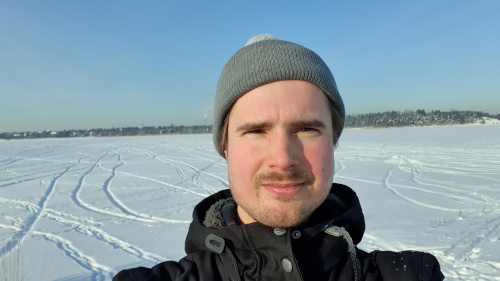
\includegraphics[width=\linewidth]{me1.jpg}
  \caption{Me in my beloved home town Helsinki in the middle of summer (well, technically in Espoo, Otaniemi)}
\end{figure}

\subsection{Education}
\begin{itemize}
\item 2016 Bachelor of Science University of Helsinki\\
\item 2018 Master of Philosophy University of Helsinki
\end{itemize}
\subsection{Research}

\begin{itemize}
\item Downlink Coverage and Rate Analysis of Low Earth Orbit Satellite Constellations Using Stochastic Geometry
  Okati, N., Riihonen, T., Korpi, D., Angervuori, I. Wichman, R., Aug 2020, In : IEEE Transactions on Communications. 68, 8, p. 5120-5134 9079921.\\
\item A. Yastrebova et al., "Theoretical and Simulation-based Analysis of Terrestrial Interference to LEO Satellite Uplinks," GLOBECOM 2020 - 2020 IEEE Global Communications Conference, Taipei, Taiwan, 2020, pp. 1-6, doi: 10.1109/GLOBECOM42002.2020.9347980.
\end{itemize}


\section{Blog posts 2021}
General thoughts on mathematics and engineering, practical instructions and artistic non sense. The themes of this blog are much inspired by challenges encountered in my professional life.

\subsubsection{January – Poisson Process on a Sphere}
Poisson process has a generalization in a large category of manifolds. Particularly Poisson point process on a sphere is useful. Nicely enough, Poisson process on a sphere is equivalent to process in a two dimensional area $ A = [-\pi,\pi] \times [-1,1]$ through the area preserving mapping from $A$ to surface of a sphere
\begin{equation}
  (x,y) \mapsto (r,x,\sin(y)) \nonumber.
\end{equation}


Resulting process interpreted in geographical coordinates $(r,\theta,\varphi)$ is a Poisson point process on a sphere of radius $r$.  Following codes returns a scatter plot of Poisson points on the unit sphere.



GNU/Octave or Matlab:
\begin{verbatim}
%Plot random points on a unit sphere. Returns the points in a vector ref in cartesian coordinates
function refc = poissononsphere(density)
  yMin = -1; yMax = 1;
  xMin=-pi; xMax = pi;
  
  xDelta=xMax-xMin;yDelta=yMax-yMin; %Rectangle dimensions
  numbPoints=poissrnd(density);    %Number of points in the area is a Poisson variable of intensity given as density
  x=xDelta*(rand(numbPoints,1))+xMin;    %Pick points from uniform distribution
  y=yDelta*(rand(numbPoints,1))+yMin;    %Map referencepoints to geographical coordinates
  ref = [x y]';

  refs = [x'; asin(y)'];%Map geographical coordinates to Cartesian coordinates on a unit circle
  r = 1;
  refc = [r*sin(refs(2,:)+pi/2).*cos(refs(1,:)+pi);...
          r*sin(refs(2,:)+pi/2).*sin(refs(1,:)+pi);...
          r*cos(refs(2,:)+pi/2)];

  figure(1)    %Plot
  [X, Y, Z] = sphere;
  surf(X,Y,Z,'EdgeColor','none','FaceColor','black');
  hold on
  scatter3(refc(1,:),refc(2,:),refc(3,:),10,...
           'MarkerFaceColor','yellow',...
           'MarkerEdgeColor','red');
  axis equal
end
\end{verbatim}

Python:

\begin{verbatim}
import numpy as np
import scipy.stats
import matplotlib.pyplot as plt
from mpl_toolkits.mplot3d import axes3d

#Rectangle dimension
xMin=-np.pi;xMax=np.pi;
yMin=-1;yMax=1;
xDelta=xMax-xMin;yDelta=yMax-yMin; #rectangle dimensions

#Density parameter of the Poisson point process. Mean number of points on the sphere
lambda0=1000; 

#Simulate Poisson point process

#Number of point in the area is a Poisson variable of intensity lambda0
numbPoints = scipy.stats.poisson( lambda0 ).rvs()
x = xDelta*scipy.stats.uniform.rvs(0,1,((numbPoints,1)))+xMin
y = yDelta*scipy.stats.uniform.rvs(0,1,((numbPoints,1)))+yMin

#Transform to geographical coordinates
x = x
y = np.arcsin(y)
#Plotting
fig = plt.figure()
ax = plt.axes(projection="3d")
ax.scatter(np.sin(y+np.pi/2)*np.cos(x+np.pi),np.sin(y+np.pi/2)*np.sin(x+np.pi),np.cos(y+np.pi/2), color='r' )
plt.show()
  
\end{verbatim}

Wolfram Language:
\begin{verbatim}
(*lambda is the mean number of points on the unit sphere*) 
  poissononsphere[lambda_] := 
  Module[{nrofpoints, phi, theta, radius, refc, polarp}, 
   nrofpoints = RandomVariate[PoissonDistribution[lambda]];
   polarp = 
    Table[{RandomVariate[UniformDistribution[{-Pi, Pi}]], 
      ArcSin[RandomVariate[UniformDistribution[{-1, 1}]]]}, 
     nrofpoints];
   radius = 1;
   refc = 
    Table[{radius*Sin[polarp[[i]][[2]] + Pi/2]*
       Cos[polarp[[i]][[1]] + Pi],
      radius*Sin[polarp[[i]][[2]] + Pi/2]*Sin[polarp[[i]][[1]] + Pi],
      radius*Cos[polarp[[i]][[2]] + Pi/2]}, {i, nrofpoints}];
   refc
   ];
   ListPointPlot3D[poissononsphere[500], BoxRatios -> {1, 1, 1}]  
\end{verbatim}

\begin{figure}
  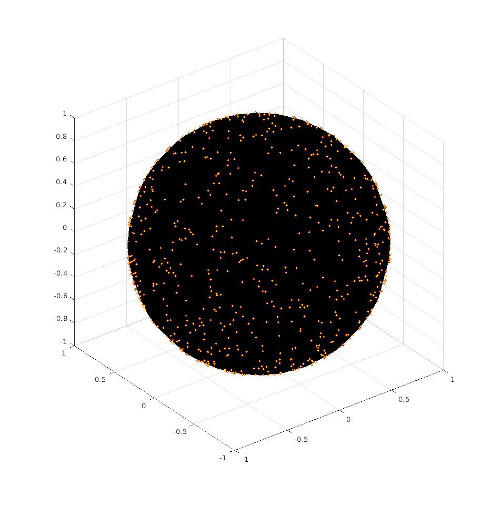
\includegraphics[width=\linewidth]{poissononsphere.jpg}
  \caption{Are the stars Poisson distributed in the sky?}
\end{figure}

\begin{figure}
  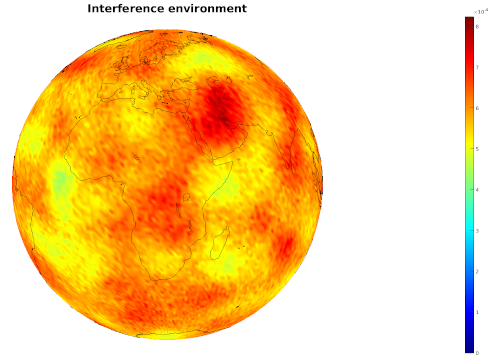
\includegraphics[width=5cm]{interferenceenvironment.png}
  \caption{Poisson distributed transmitters and the aggregate signal strength in a satellite by location. Poisson assumption is reasonable in varying situations, but, well, here the sea areas are a bit overrepresented.  }
\end{figure}

References:
\bibitem{theoryofpoint} D. J. Daley and D. Vere-Jones, ``The General Poisson Process'' in {\em An introduction to the theory of point processes.} New York: Springer, 2003, pp. 39. 
\bibitem{2} Stoyan, Dietrich. et al. \em{Stochastic Geometry and Its Applications}. 3rd ed. Chichester: Wiley, 2013. Print.




\subsection{February – Controlling your Passwords with Pass}
Pass is a nice unix style free and open source wallet for keeping your passwords safe. Here is a brief look how to set it up in Ubuntu.

\begin{itemize}
\item Install the application in the terminal \\
\begin{verbatim}
sudo apt install pass  
\end{verbatim}
\item Check for existing GPG keys \\
\begin{verbatim}
gpg --list-keys 
\end{verbatim}
\item If no keys were found generate a key pair \\
\begin{verbatim}
gpg --generate-key
\end{verbatim}
\item Copy the name of the key and initialize pass\\
\begin{verbatim}
pass init ABCDEFGHIJKLMNOPQRSTUV1234, 
\end{verbatim}
where ABCDEFGHIJKLMNOPQRSTUV1234 is the name of the key.
\item Generate a password with \\
\begin{verbatim}
pass generate keyfolder/newkey 
\end{verbatim}
List passwords
\begin{verbatim}
pass
\end{verbatim}
Copy a password to clipboard \\
\begin{verbatim}
pass keyfolder/newkey -c
\end{verbatim}
For more commands
\begin{verbatim}
man pass
\end{verbatim}
\end{itemize}

Connect pass to git so it is easy to keep track of changes with multiple machines.

\begin{itemize}
\item Export your public and private key to a file with \\
  \begin{verbatim}
gpg --export --output public.key ABCDEFGHIJKLMNOPQRSTUV1234 
gpg --export-secret-key --output private.key ABCDEFGHIJKLMNOPQRSTUV1234,
  \end{verbatim}
  where ABCDEFGHIJKLMNOPQRSTUV1234 is your key name.\\
\item Now we can initialize the git repository with these keys. Move public.key and private.key through a safe channel to a computer you wish to use pass in. Import the keys to the machine \\
\begin{verbatim}
gpg --import public.key
gpg --import private.key
\end{verbatim}
\item After importing keys to a new machine you can initialize pass
\begin{verbatim}
pass init ABCDEFGHIJKLMNOPQRSTUV1234
\end{verbatim}

\item Initialize your git repository. Make a new repository named pass-store e.g. to GitHub if you are doing this first time before the following commands\\
\begin{verbatim}
pass git init 
pass git remote add origin git@repo.com:myname/pass-store
 \end{verbatim}
\item Get password data from the server (from a non-empty repository, otherwise skip)
\begin{verbatim}
pass git pull origin master --allow-unrelated-histories
pass git commit -am "firstcommit"
\end{verbatim}
\item Do some changes and pass will automatically commit them. Push and set upstream \\
\begin{verbatim}
pass git push --set-upstream origin master 
\end{verbatim}
\item From here on you can use the familiar git commands \\
\begin{verbatim}
pass git pull 
pass git push 
\end{verbatim}
\end{itemize}
Stay safe :)


References:

\bibitem[1]{pass}\htmladdnormallink{Password Store}{\pass}


  \subsection{March – Signal Propagation in a City}
  People in the city trying to contact their fellow mates by cell phones will have to exchange data by electromagnetic waves with their base stations. This data is relevant only to the parties communicating with each other. As some of the data signals gets leaked to the surroundings, each transmission will cause an interference field, which will disturb other transmissions in the same frequency band.

  Interference in big crowds gets so large that data transmission rates will lower to the level of jamming. This shows for example in crowded festival areas as difficulties to reach out your friend by your mobile phone.

  \begin{figure}
  \includegraphics[width=\linewidth]{rician.gif}
  \caption{Interference field developing in time. We assume random multi path signal propagation from random locations moving to random directions in time. Also, a line-of-sight component is present. Red occurrences will cause remarkable disturbance in communication.}
\end{figure}


  References:

\bibitem[1]{hurr}François Baccelli, Bartlomiej Blaszczyszyn \htmladdnormallink{Stochastic Geometry and Wireless Networks, Volume I -Theory}{\hal}

  \subsection{April – Frequentist Inference in Mathematica}
  Mathematica provides a package called ``Hypothesis Testing'' for analyzing random data. Package includes handy objects like ``Around'' which represents an quantity and the uncertainty around it. Following example code returns an Around object representing the $90 \%$ confidence interval of the estimated bias of a coin after a repeated trial. Like shown in the code, the ListPlot plots Around objects as such.


\begin{verbatim}
(*Load the Hypothesis Testing Package.*)
Needs["HypothesisTesting`"];

coin[flips_, bias_] :=
 (*Make the experiment and collect the data*) 
 Module[{index, realizations, mean, conf, around},
  realizations = {};
  For[index = 1, index <= flips, index++,
   realizations =  
     Append[realizations, 
      RandomVariate[BernoulliDistribution[bias]]];
   ];
  
  (*Means*)
  mean = Mean[realizations[[All]]];
  (*Confidence intervals*)
  conf = MeanCI[realizations[[All]]];
  (*Around object.*)
  
  around = Around[mean, Abs[conf[[1]] - conf[[2]]]]
  ]
coin[1000, 0.5]
ListPlot[{
Around[0.488, 0.0620678530067702]}]
\end{verbatim}

  
  
  
 
  
   
\end{document}
%
% optional post-title formatting for PostScript
%
\parindent0pt
\parskip2.5ex plus 0.5ex minus 0.5ex

